\documentclass[onecolumn, draftclsnofoot, 10pt, compsoc]{IEEEtran}
\usepackage{url}
\usepackage{setspace}
\usepackage[english]{babel}
\usepackage{hyperref}
\usepackage{graphicx}
\usepackage{float}
\usepackage[margin=0.75in]{geometry}
\usepackage[justification=centering]{caption}
\usepackage{pythonhighlight}

\newenvironment{myitemize}
{ \begin{itemize}
    \setlength{\itemsep}{0pt}
    \setlength{\parskip}{0pt}
    \setlength{\parsep}{0pt}     }
{ \end{itemize}                  }

\def\code#1{\texttt{#1}}
% 1. Fill in these details
\def \CapstoneTeamName{Code Monkeys in Space}
\def \CapstoneTeamNumber{		33}
\def \GroupMemberOne{			Mark Bereza}
\def \GroupMemberTwo{			Joseph Struth}
\def \GroupMemberThree{			Kevin Turkington}
\def \CapstoneProjectName{		NASA University Student Launch Initiative}
\def \CapstoneSponsorCompany{	Mechanical Engineering, Oregon State University NASA}
\def \CapstoneSponsorPerson{		Dr. Nancy Squires}

% 2. Uncomment the appropriate line below so that the document type works
\def \DocType{	%	Technology Review and Implementation Plan
				%Requirements Document
				%Technology Review
				%Design Document
				Progress Report
				}
			
\newcommand{\NameSigPair}[1]{\par
\makebox[2.75in][r]{#1} \hfil 	\makebox[3.25in]{\makebox[2.25in]{\hrulefill} \hfill		\makebox[.75in]{\hrulefill}}
\par\vspace{-12pt} \textit{\tiny\noindent
\makebox[2.75in]{} \hfil		\makebox[3.25in]{\makebox[2.25in][r]{Signature} \hfill	\makebox[.75in][r]{Date}}}}
% 3. If the document is not to be signed, uncomment the RENEWcommand below
\renewcommand{\NameSigPair}[1]{#1}

\definecolor{stratosphere}{HTML}{006A8E}

\hypersetup{pdfauthor={Mark Bereza, Joseph Struph, Kevin Turkington},
	colorlinks   = true,
	urlcolor     = stratosphere,
	linkcolor    = stratosphere
}

%%%%%%%%%%%%%%%%%%%%%%%%%%%%%%%%%%%%%%%
\begin{document}
\begin{titlepage}
    \pagenumbering{gobble}
    \begin{singlespace}
    	%%\includegraphics[height=4cm]{coe_v_spot1}
        \hfill 
        % 4. If you have a logo, use this includegraphics command to put it on the coversheet.
        %\includegraphics[height=4cm]{CompanyLogo}   
        \par\vspace{.2in}
        \centering
        \scshape{
            \huge CS Capstone \DocType \par
            {\large\today}\par
            \vspace{.5in}
            \textbf{\Huge\CapstoneProjectName}\par
            \vfill
            {\large Prepared for}\par
            \Huge \CapstoneSponsorCompany\par
            \vspace{5pt}
            {\Large\NameSigPair{\CapstoneSponsorPerson}\par}
            {\large Prepared by }\par
            Group\CapstoneTeamNumber\par
            % 5. comment out the line below this one if you do not wish to name your team
            \CapstoneTeamName\par 
            \vspace{5pt}
            {\Large
                \NameSigPair{\GroupMemberOne}\par
                \NameSigPair{\GroupMemberTwo}\par
                \NameSigPair{\GroupMemberThree}\par
            }
            \vspace{20pt}
        }
        \begin{abstract}
        % 6. Fill in your abstract    
        	This document serves as a retrospective of all work done to the website, avionics DLM, and rover over the spring term.
        \end{abstract}     
    \end{singlespace}
\end{titlepage}
\newpage
\pagenumbering{arabic}
\tableofcontents
% 7. uncomment this (if applicable). Consider adding a page break.
%\listoffigures
%\listoftables
\clearpage

% 8. now you write!
\section{Purposes and Goals}
Overall, the goals of this competition are the following:
\begin{enumerate}
\item Construct and launch a rocket carrying a payload at least a mile (5,280 feet) above ground.
\item Have the rocket deploy a parachute and safely land within 2,500 feet of the launch point.
\item After landing and after a button press, deploy a rover.
\item Have the rover drive autonomously at least 5 feet away from the rocket landing site.
\item Have the rover deploy solar cells after being at least 5 feet from the landing site.
\item The solar cells will increase in surface area after deployment (unfold).
\item Create formal technical reports regarding rocket/payload design and present them to a NASA review panel
during several formal design review meetings.
\item Participate in educational outreach sessions and get at least 200 students involved in STEM subjects.
\item Maintain a website detailing project information and hosting all competition deliverables.
The subset of these overall goals that pertain to the CS capstone students involves the research, design, implementation.
\end{enumerate}
In particular, the CS seniors on the OSU USLI team, otherwise known as Code Monkeys in Space, are responsible for goal 9, their shares of goals 7 and 8, and the software needed to facilitate goals 4 and 5. Furthermore, Code Monkeys in Space are responsible for the design and implementation of software that will track the drift of the launch vehicle sections, which indirectly assist with goals 1 and 2. Thus, the scope of this project for Code Monkeys in Space is limited to these facets of the competition. The others will be handled by the mechanical and electrical engineering seniors on the team. If every subteam successfully completes their responsibilities in a timely, complete, and safe manner, the team as a whole will accomplish the overall goal of scoring well in this competition.

\section{Progress Thus Far}

\subsection{USLI Competition Results}
\textbf{Source: OSU-USLI-2018 PLAR}\par
The competition flight was almost fully successful with two failures.  Both sections drifted just outside of the allowable drift radius, and the rover was not successfully deployed.  All other NASA and team derived requirements were met.

The other concern from the flight is that the motor appeared to be underpowered, like our second full-scale flight. The rocket was stable off the launch pad but began wind cocking while coasting to apogee. The rocket reached an altitude of 3355 ft. which was 1527 ft. lower than expected and 1948 ft. lower than the target altitude. In addition, the maximum velocity was 132 ft./s lower than expected.  This is attributed to low initial thrust and poor-quality control of the L850W  motor selected. The rocket off the launch pad is shown in Figure \ref{figure: Comp Launch}

\begin{figure}[H]
	\centering
	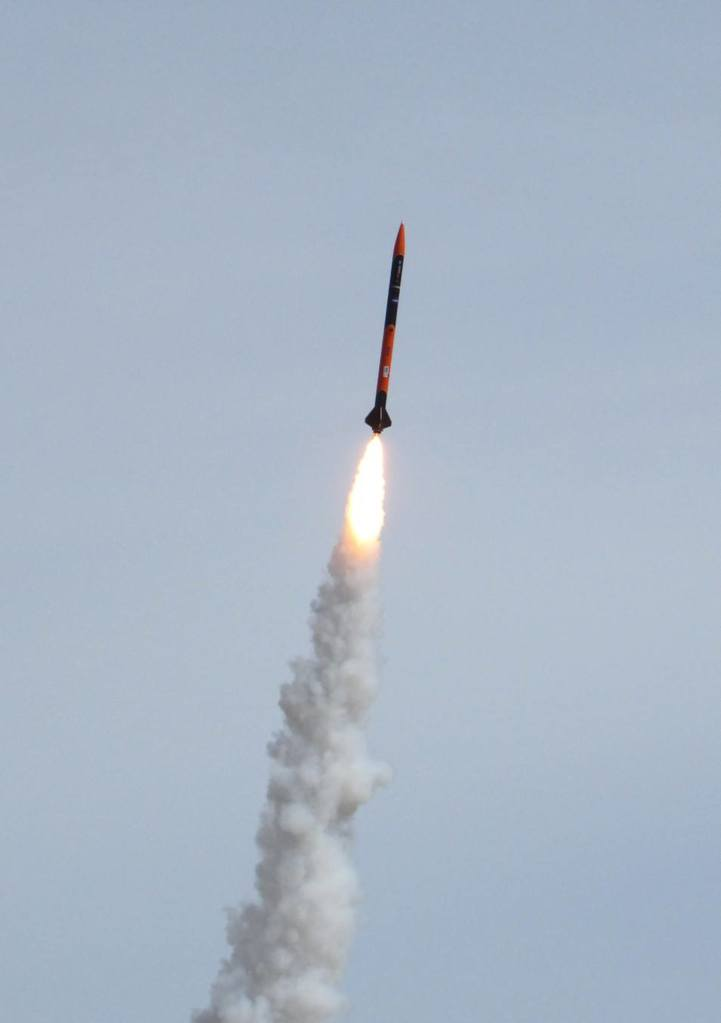
\includegraphics[width=0.7\textwidth]{competitionlaunch_1024.jpg}
	\caption{Competition Launch}
    \label{figure: Comp Launch}
\end{figure}

The fore section main parachute opened as expected, but the descent rate under main was slower than in both previous flights and simulations.  It drifted out of the allowed area to the edge of a group of trees.  It was found 2572 ft. away tangled in a tree about 15 ft. off the ground, but damage to limbs above where it was found suggested it bounced off a couple higher trees before coming to rest.  The fore section can be seen where it was found in Figure \ref{figure: Fore Land}.  The main parachute had a few large tears that will have to be patched before it can be used again.

\begin{figure}[H]
    \begin{minipage}{0.5\textwidth}
        \centering
        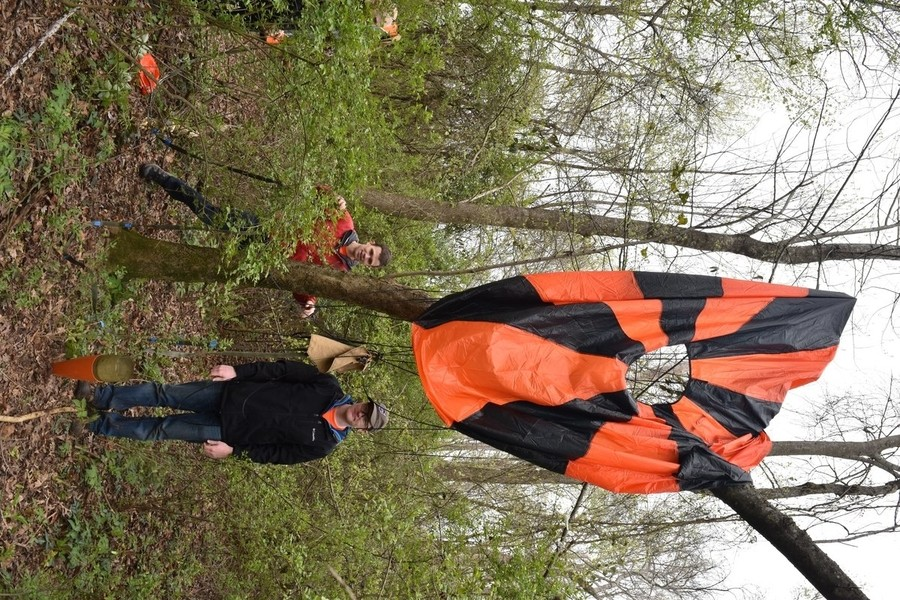
\includegraphics[width=\textwidth,angle=90]{fore_landing.jpg}
	    \caption{Landed Fore Section}
        \label{figure: Fore Land}
    \end{minipage} \hfill
    \begin{minipage}{0.5\textwidth}	
        \centering
        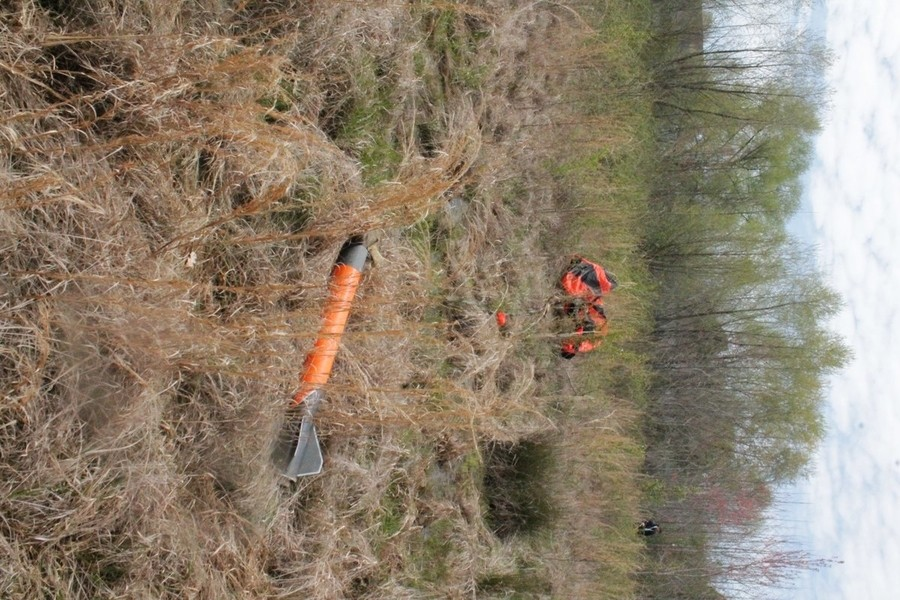
\includegraphics[width=\textwidth,angle=90]{aft_landing.jpg}
	    \caption{Landed Aft Section}
        \label{figure: Aft Land}
    \end{minipage}
\end{figure}

The aft section had its main parachute slip out of the Jolly Logic Chute Release at around 1900 ft., 900 ft higher than expected. It drifted past the fore section where it landed high in a tree next to a swamp where the land owner of Bragg Farm was. According to him, the wind pulled the aft section out of the tree and it landed in the swamp, 3511 ft. away from the launch pad, where it was easily recovered. The aft section can be seen where it was found in Figure \ref{figure: Aft Land}. There was no damage to any of the components.

\begin{itemize}
\item The team as a whole has already exceeded the
education outreach minimum requirement of 200.
Currently the USLI team has reached 900 students total!

\item Critical Design Review score sheets are in; OSU USLI
team finished in the top 2\% in the competition which
equates to 1st out of 50 teams! This result is very good
for a first year rookie team. CS Team members
contributed to the 250 page document by formatting and
adding sections written by other capstone team
members in \LaTeX.

\item The team performed well at the Competition April 4th-9th IN Huntsville, AL. Winning third place in the payload design category. Since one of the top three payload designs was a target detection system, this meant OSU's USLI team had the second best rover design at the competition!
\end{itemize}

\subsection{Launch Readiness Review}
Besides the actual competition launch, Code Monkeys in Space also joined the rest of the OSU USLI team in participating in the Launch Readiness Review (LRR) prior to the launch. The purpose of the LRR was to evaluate whether the team's launch vehicle was ready for launch and met all safety requirements. This was done by the team disassembling the launch vehicle in front of a panel of safety inspection officers and describing the function and parameters of each systems, which can be seen in Figure \ref{figure:Launch Readiness Review}. Overall, the team passed the LRR with only one assembly procedure change requested by the safety officers concerning safety equipment worn during the loading of black powder charges.

\begin{figure}[H]
	\centering
	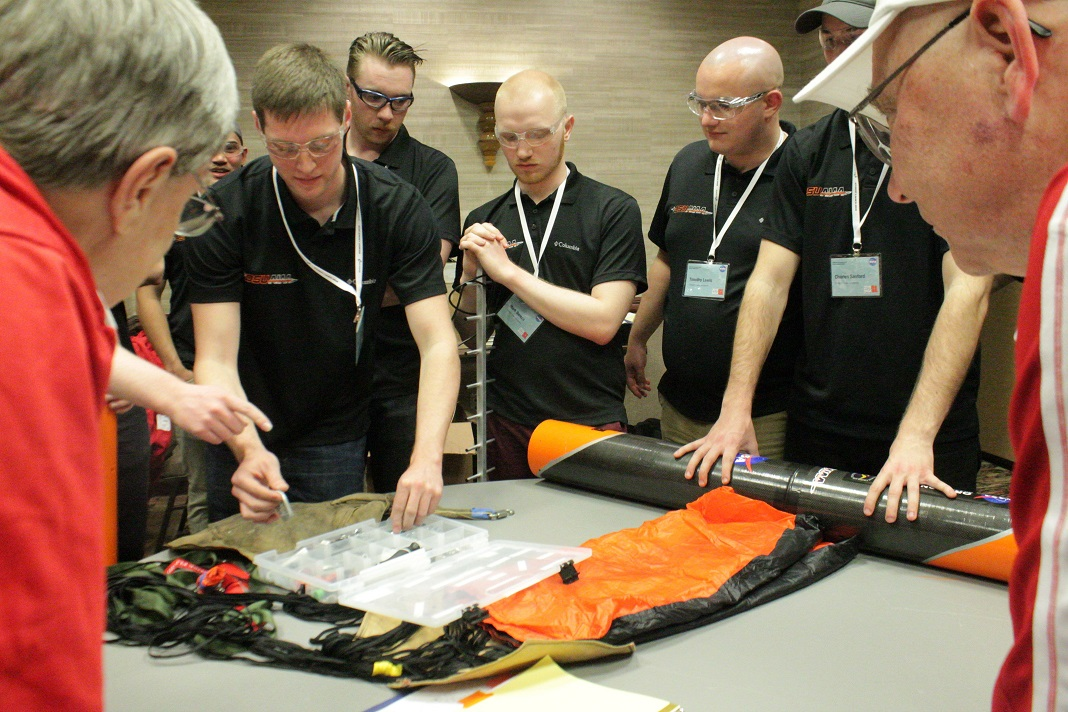
\includegraphics[width=0.8\textwidth]{LRR.jpg}
	\caption{OSU's USLI Team at the Launch Readiness Review}
    \label{figure:Launch Readiness Review}
\end{figure}

\subsection{Post Launch Assessment Review}
The PLAR was completed, submitted, and sent to NASA April 26. The document is the final written deliverable for the competition and briefly recounted the results of the launch in Alabama, along with analysis for all points of failure and lessons learned over these last eight months. Mark Bereza assisted with formatting of the document's tables, editing the report for errors, and posting the completed document on the team website.

\subsection{Educational Outreach}
The team as a whole conducted several educational outreach events, with each member of Code Monkeys in Space participating in at least two events. Although the larger team conducted two more outreach events during spring term, Code Monkeys in Space did not participate in these particular events. The team as a whole has already exceeded the education outreach minimum requirement of 200. Currently the USLI team has reached almost 1000 students total!

\subsection{Rover}
During the competition in Huntsville, Alabama ejection of the rover payload failed because the Payload Ejection Controller (PLEC) ran out of battery by the time the signal for deployment was sent to the aft section, which housed the payload. This is because the PLEC's batteries were only rated for about 6-8 hours and over six hours had passed between powering on the PLEC before launch and the successful recovery and retrieval of the aft section. The long delay between the two was a result of the aft section landing in the trees over half a mile from the launch site, making recovery tedious. However, when the rover was removed manually from the launch vehicle, it successfully drove at least five feet from the launch vehicle and deployed solar panels autonomously (Figure \ref{figure:Rover at Competition}), thus meeting all the payload requirements for this project.

\begin{figure}[H]
	\centering
	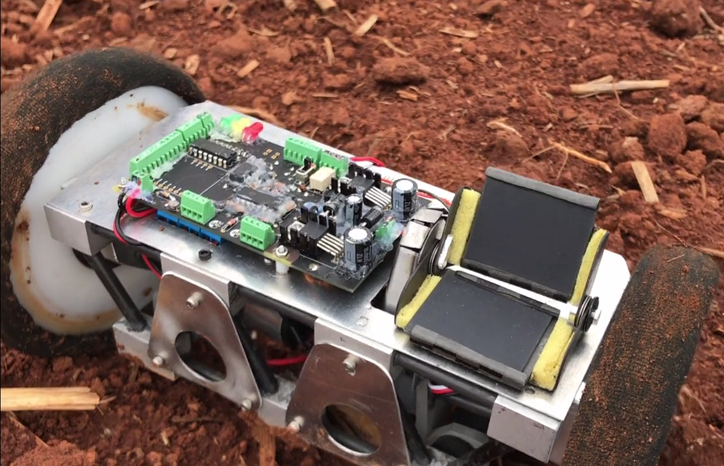
\includegraphics[width=0.8\textwidth]{rover.png}
	\caption{Rover at Competition, After Deploying Solar Panels}
    \label{figure:Rover at Competition}
\end{figure}

\subsection{Ground Station and Launch Vehicle Tracking}

\begin{figure}[H]
	\centering
	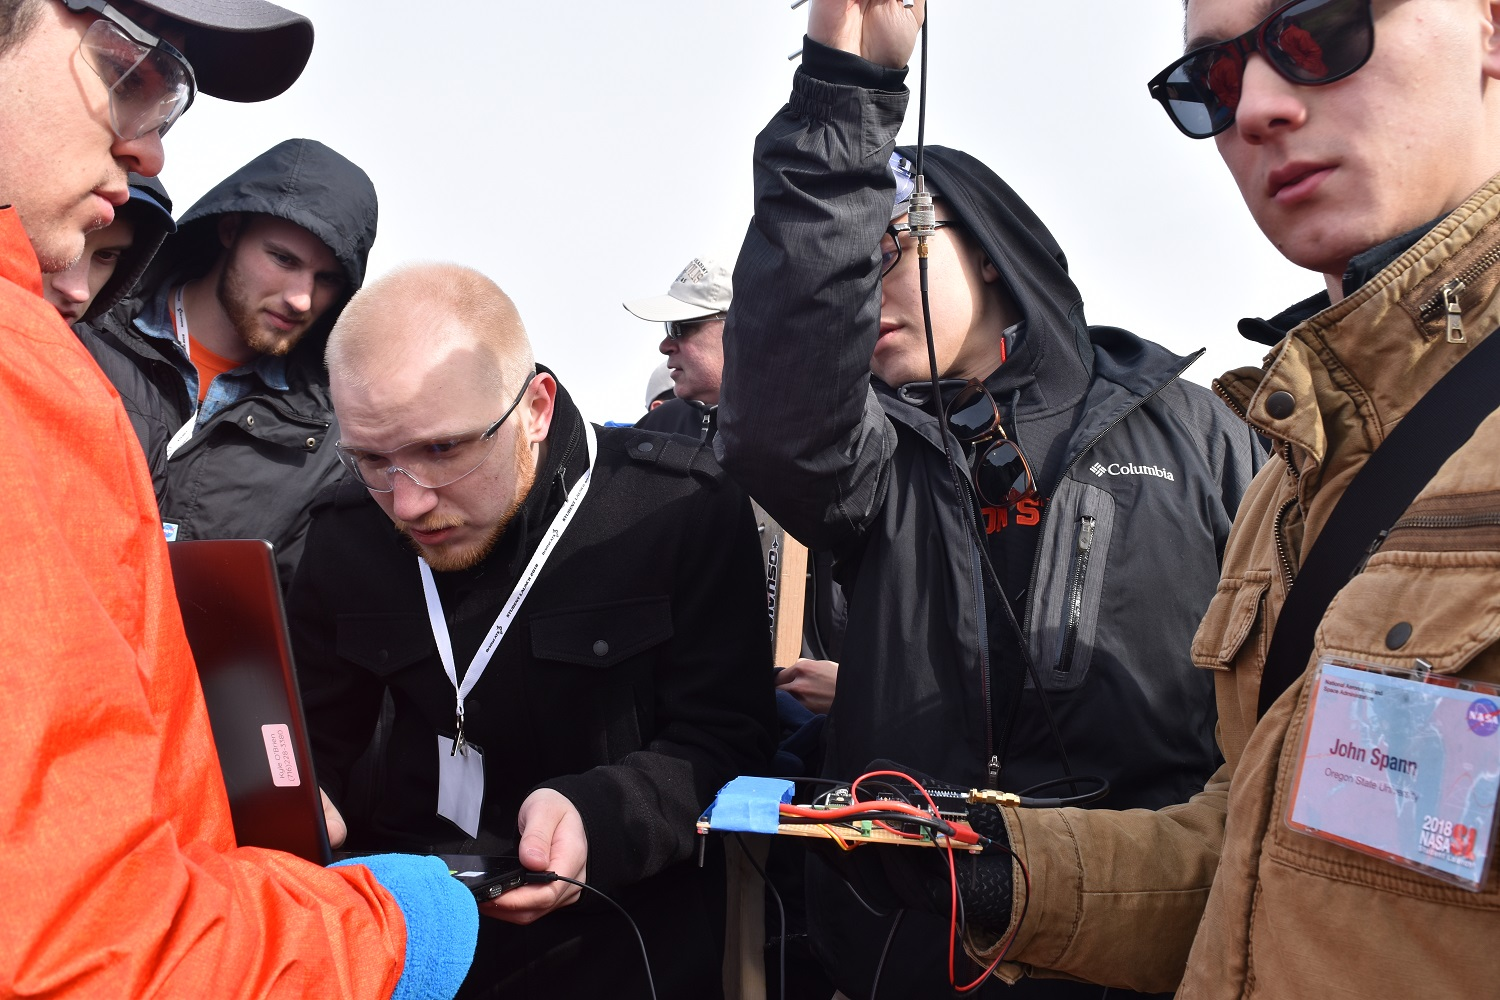
\includegraphics[width=0.8\textwidth]{ground_station.JPG}
	\caption{Ground Station During Competition}
    \label{figure:Ground Station}
\end{figure}

Although the software for the ground station was working during the competition in Alabama and the receiving antenna connected to the ground station depicted in Figure \ref{figure:Ground Station}, was briefly able to lock onto and communicate with the GPS sending antennas onboard the launch vehicle, there was ultimately too much RF interference at the competition grounds to successfully track the launch vehicle during its flight. This was due to other teams broadcasting at multiple frequencies and at higher power than allowed by the competition rules. Ultimately, Code Monkeys in Space successfully met the software requirements for the ground station and there was little that could have been done to prevent the tracking failure on the software side of things. The ground station software, which plots the drift of the launch vehicle using received GPS data, can be seen running in Figure \ref{figure:Ground Station 2}.

\begin{figure}[H]
	\centering
	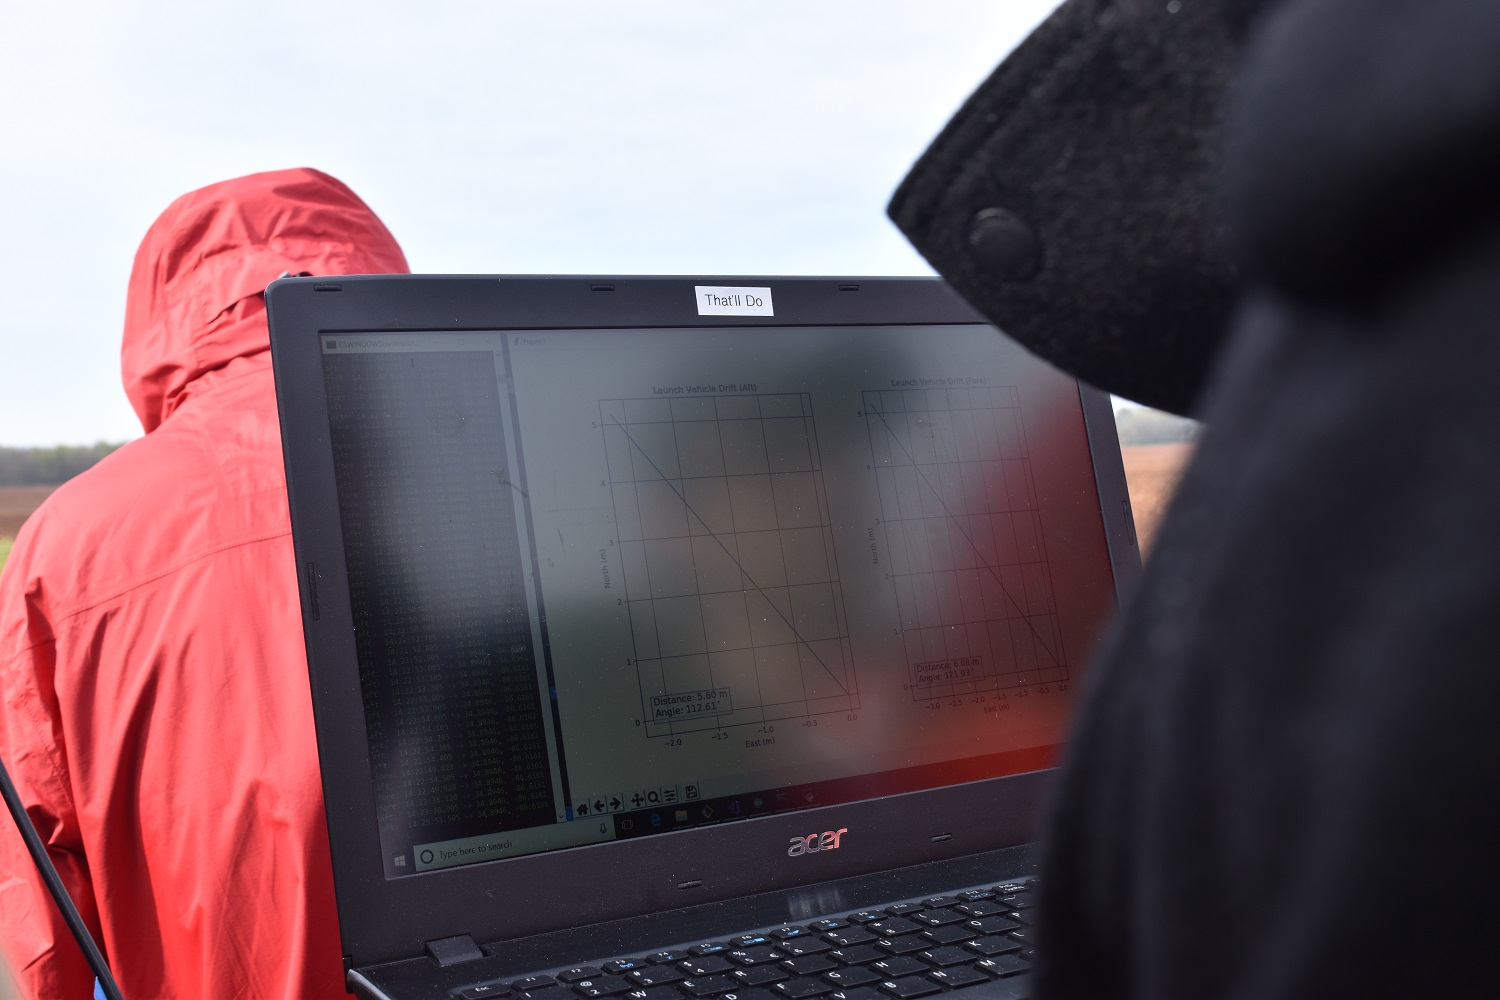
\includegraphics[width=0.8\textwidth]{ground_station_2.JPG}
	\caption{Ground Station Software Communicating With Launch Vehicle on Launch Pad}
    \label{figure:Ground Station 2}
\end{figure}

\subsection{Website}
The team has kept the website up to date with NASA document deliverables, posting FRR, and PLAR documents and fly sheet documents on the website available for download by NASA. No other changes have been needed as the website was otherwise complete by the end of winter term.

\section{Work Left to do}

\subsection{Rover}
The rover is complete, performed well at competition, and the team won third place in payload design for all the hard work put into it. The remaining work to do for the rover is presenting the project and displaying the rover at engineering expo on May 18 alongside the electrical and mechanical engineering teams. Additionally, minor documentation of the mains scripts and systems used by the computer science team will have to be made for expo. Although it is not part of the competition requirements, Mark Bereza is also going to assist the electrical engineering team members in fully integrating the sonar sensors with the rover to help them meet their capstone requirements and to make the rover a little more impressive for expo.

\subsection{Ground Station and Launch Vehicle Tracking}
The ground station software is complete and functioned fully during competition, only failing to track the launch vehicle due to RF interference.

\subsection{Website and Competition Deliverables}
The website is complete in terms of functionality and presentation and all NASA deliverables have been posted, so there is no work left to do for it.

\section{Stumbling Blocks and Solutions}
\subsection{General}
\begin{itemize}
\item Problem: Team members submitting and editing content for the FRR at the last minute.
\begin{itemize}
\item Solution: Extra time was allotted by the team lead for the CS Team to format the document. 
\end{itemize}
\item Problem: CS Team attending engineering specific meetings taking up much needed development time during the week.
\begin{itemize}
\item Solution: Communicated with team leads, and agreed to communicate via slack if attendance or input is needed at a meeting. This allowed the CS team to meet 3 times a week to continue development.
\end{itemize}
\end{itemize}

\subsection{Rover}
\begin{itemize}
\item Problem: Knowledge gap for electrical engineering as applied to sensors and embedded programming.
\begin{itemize}
\item Solution: Collaborate closely with the electrical engineers on the rover sub team to assist with sensors and drivers.
\end{itemize}
\item Problem: Some Raspberry Pi pins were burnt and rendered unusable.
\begin{itemize}
\item Solution: Members of the team immediately purchased additional controllers for the electrical and computer science team members.
\end{itemize}
\item Problem: Test bed disassembled by mechanical engineers when needed for testing by EE and CS team.
\begin{itemize}
\item Solution: Work together with ME and EE sub teams to reassemble test bed and prepare it for motor driver and sonar testing.
\end{itemize}
\item Problem: Monitor, keyboard, and mouse were usually not available for accessing the Raspberry Pi, and this became a non-option later on when the Pi was integrated into the rover and attaching such peripherals would be impossible.
\begin{itemize}
\item Solution: A laptop would SSH into the Raspberry Pi by connecting to it via an ethernet cable, bridging the connection with the connected WiFi network, and running WireShark with the "arp" filter to discover the IP address of the Raspberry Pi.
\end{itemize}
\end{itemize}

\subsection{Ground Station}
\begin{itemize}
\item Problem: Unable to perform proper range testing for the ground station communication antenna due to the ground clipping the signal cone.
\begin{itemize}
\item Solution: Drove out to a location with a large hill and performed antenna range testing from the top, thus reducing the negative effect of ground clipping.
\end{itemize}
\item Problem: The receiving antenna for the ground station is uncomfortable to hold for long periods of time but the GPS modules require a long time to get a GPS lock.
\begin{itemize}
\item: Solution: A wooden "gun stock", depicted in Figure \ref{figure:Gun Stock}, was added to the receiving antenna to make it more comfortable to hold and aim accurately.

\begin{figure}[H]
	\centering
	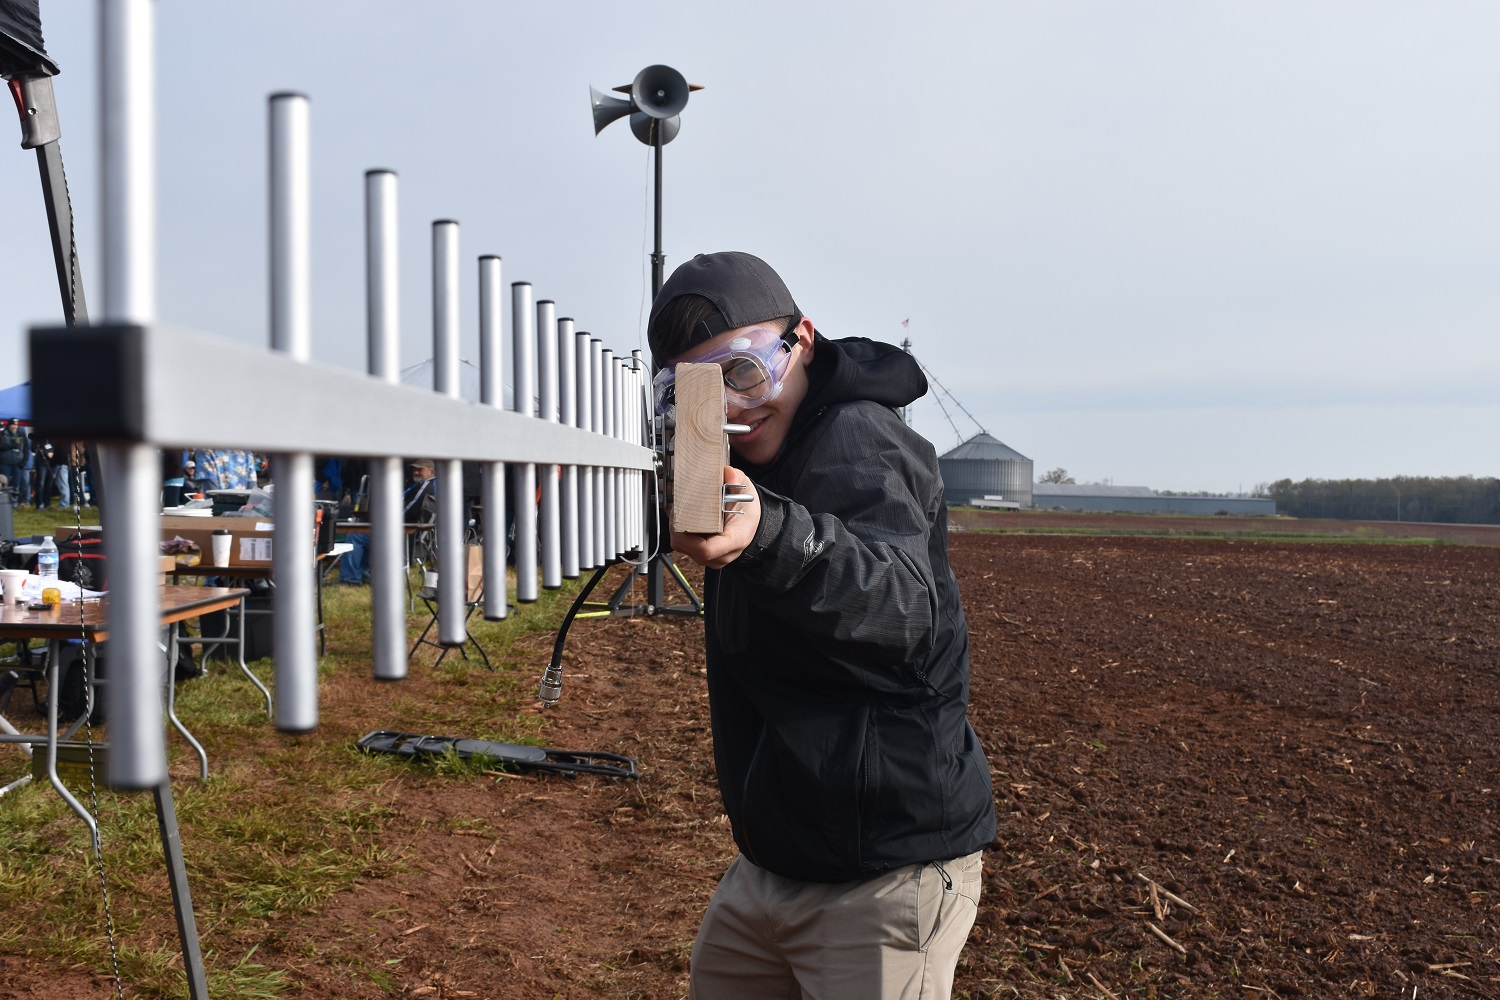
\includegraphics[width=0.8\textwidth]{gun_stock.JPG}
	\caption{Wooden "Gun Stock" That Was Added to the Ground Station Antenna Prior to Competition}
    \label{figure:Gun Stock}
\end{figure}

\end{itemize}
\end{itemize}

\subsection{Website}
\begin{itemize}
\item Problem: Vague improvement and change requests from team lead regarding website aesthetics. 
\begin{itemize}
\item Solution: Sat down for a one on one and discussed specifically what the team lead wanted.
\end{itemize}
\item Problem: Team members not submitting head shots to the "About Us" section of the website.
\begin{itemize}
\item Solution: Contact team leads to put pressure on members to meet this requirement.
\end{itemize}
\end{itemize}

\end{document}
